<<echo=FALSE, cache=FALSE>>=
set_parent('./project.Rnw')
@
%
To measure the performance and explore the how well theory and practice coincide, the methods discussed will be trained and tested on different datasets in this chapter. Some extensions will also briefly be discussed at the end.

\section{Spam dataset}
\label{sec:Spam dataset}
\colorbox{yellow}{Need to write something about the data set. Description and so on.}\\
\colorbox{yellow}{Look at what others have done.} \\
\url{http://sci2s.ugr.es/keel/dataset.php?cod=109} Spam data.\\
\\
\colorbox{yellow}{If I use categorical variables, should I include section on how the algorithms handles them?}\\
 The first dataset explored is a pretty common dataset in the machine learning world. 
 Each datapoint in the dataset corresponds to an email, with the binary response telling if an email is spam or not. There are a total of 4601 data points and 57 predictors:
 \begin{itemize}
   \item 48 continuous real $[0, 100]$ corresponding to words. Each giving the percentage of words in the email matching that word. 
   \item 6 continuous real $[0, 100]$ corresponding to characters. Each giving the percentage of characters in the email matching that characters.
   \item 1 continuous real $[1, \ldots]$ giving average length of uninterrupted sequences of capital letters. 
   \item 1 continuous integer $[1, \ldots]$ giving length of longest uninterrupted sequence of capital letters.
   \item 1 continuous integer $[1, \ldots]$ giving total number of capital letters in the email.
 \end{itemize}
 For more information on the dataset see \cite{Spamdata}.

 In the tests that follows the spam data was split into a training and test set of same size. The algorithms are first trained on the training set, and the test error in form of $0/1$ misclassification error rate is plotted, i.e.
 \begin{align}
   \label{eq:missClassErr} 
   error =  \frac{1}{n_{test}} \sum_{i = 1}^{n_{test}} I\{C(\mathbf{x}_i) \neq y_i\},
 \end{align}
 where $C(\mathbf{x}_i)$ is the prediction based on $\mathbf{x}_i$, and $n_{test}$ is the number of test points. If the goal had been to actually make a spam filter, the error measure would not weight misclassification of spam and non-spam the same. Different costs for misclassification has not been the focus of this project, but for the purpose of testing the behavior of different methods \eqref{eq:missClassErr} works well.
 

\section{CART}
\label{sec:CARTsim}
Simulation 1: \\
Plot pruned and unpruned tree. \\
Plot test error for different \verb+cp+ parameters, or (same) different pruning. From full tree, back to a stump.\\
Hope that \verb+cp+ in \verb+pruning.rpart+ is the same as $\alpha$ in cost complexity pruning??? Hei

\begin{figure}[h!]
\begin{center}
    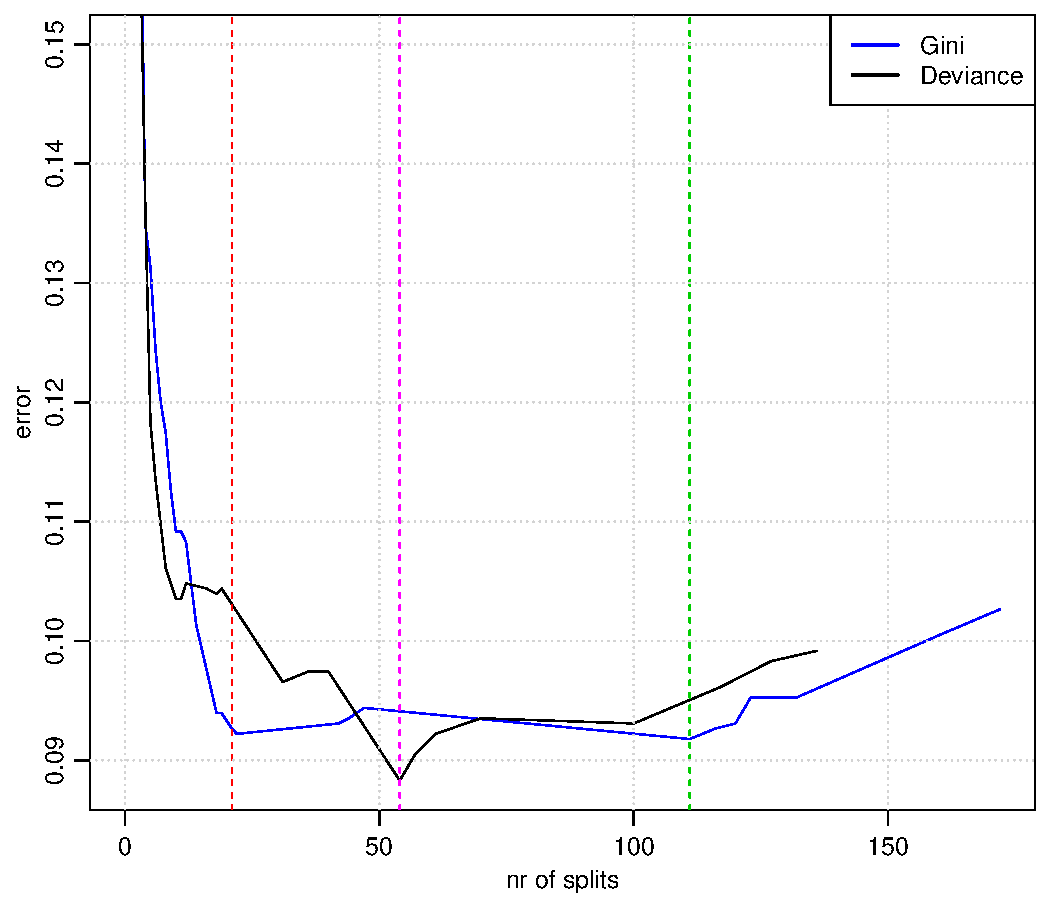
\includegraphics[scale=0.5]{./figures/cartCPSpam.pdf}
\end{center}
\caption{CART on spam data. Test error as function of number of splits. The two lines represent trees grown with ''Geni'' and ''Deviance'' splitting criteria. A large tree is grown and the different points are test error of pruned trees depending on the tuning parameter $\alpha$ in \eqref{eq:CostPruning}. The green and magenta line marks the minima for the two lines. }
\label{fig:cartCPSpam}
\end{figure}

\begin{figure}[h!]
  \centering
  \begin{subfigure}[b]{0.48\textwidth}
    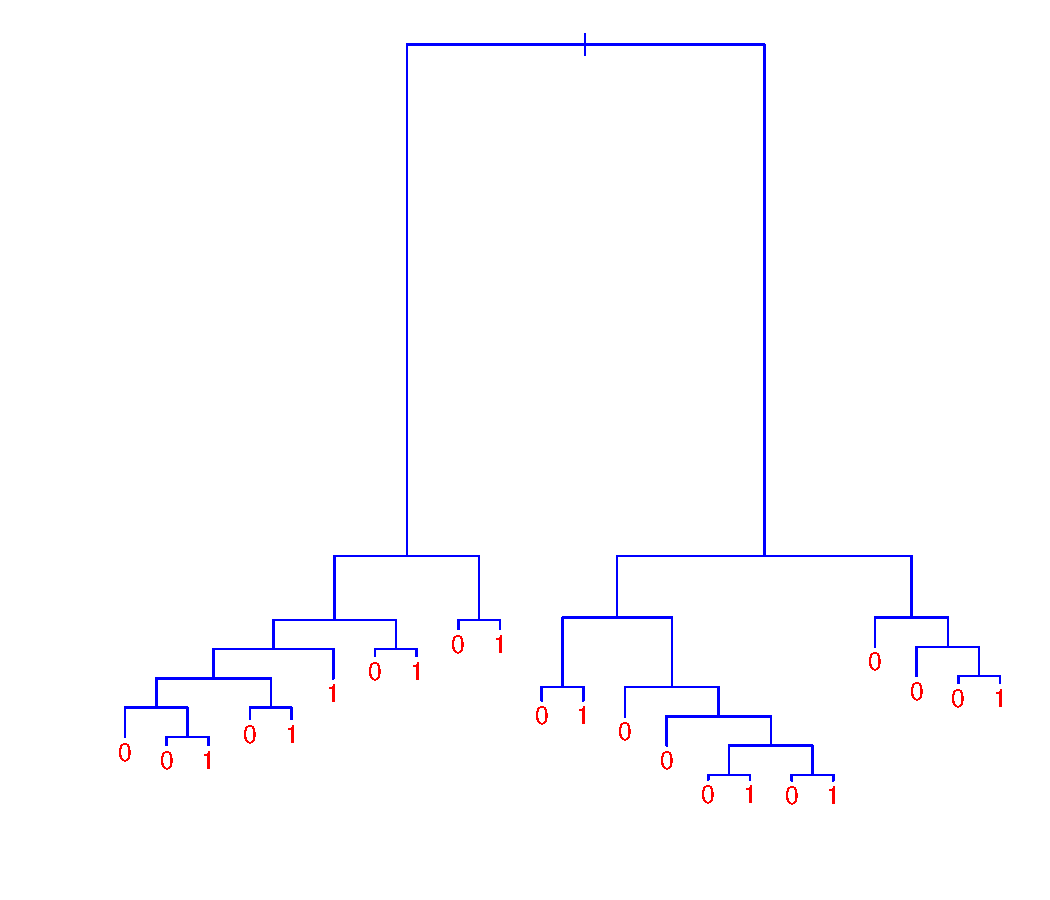
\includegraphics[width=\textwidth]{./figures/cartSmallSpam.pdf}
  \end{subfigure}%
  \quad
  \begin{subfigure}[b]{0.48\textwidth}
    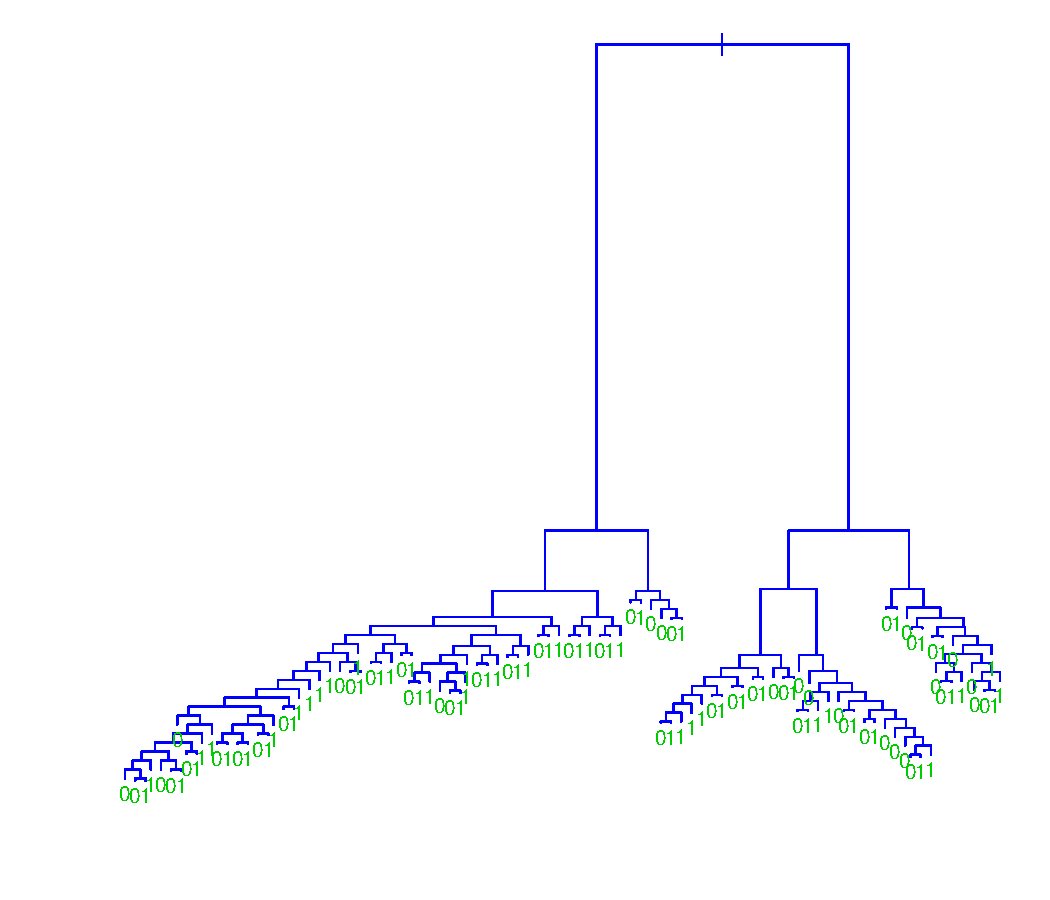
\includegraphics[width=\textwidth]{./figures/cartOptSpam.pdf}
  \end{subfigure}
  \quad
  \begin{subfigure}[b]{0.48\textwidth}
    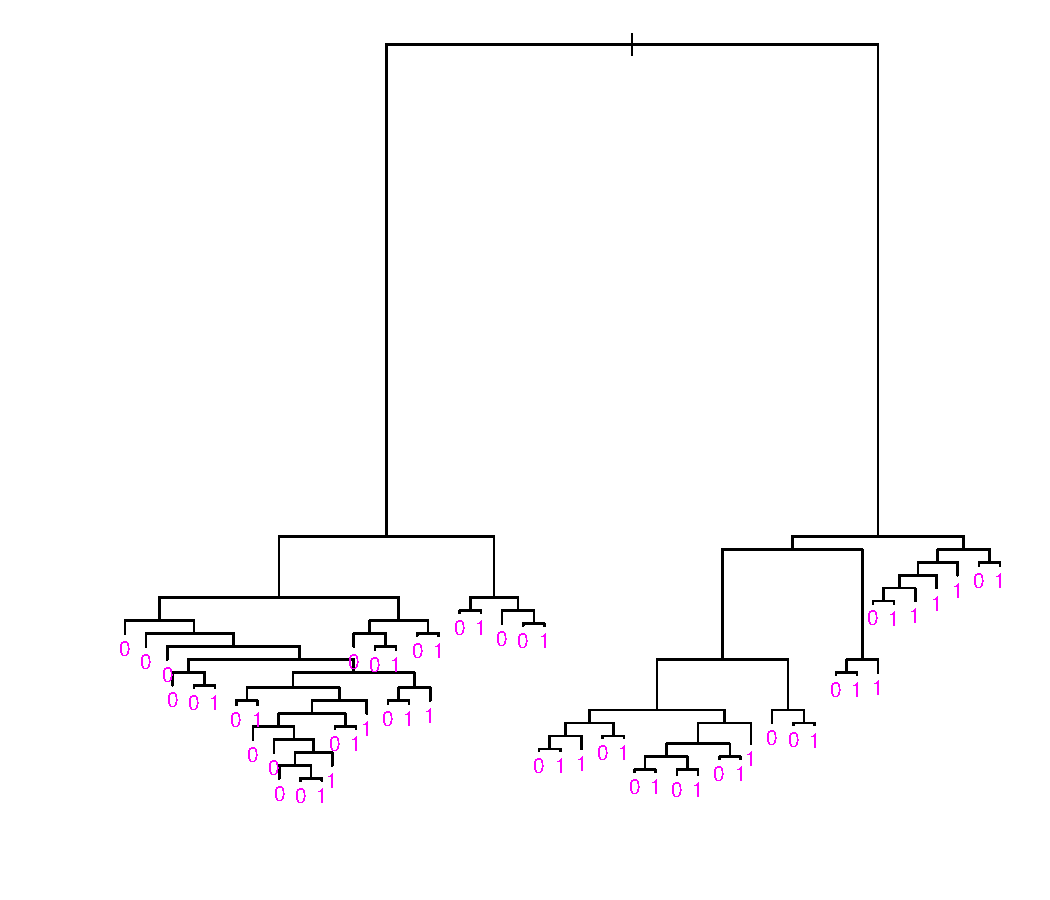
\includegraphics[width=\textwidth]{./figures/cartOptDevianceSpam.pdf}
  \end{subfigure}
          %(or a blank line to force the subfigure onto a new line)
  \vspace{1\baselineskip}
  \caption{CART on spam data. Trees from \ref{fig:cartCPSpam} are displayed. The green tree has the minimal test error using ''Ginie'' splitting, while the red have a much simpler structure with almost the same test error. The magenta tree is the best performing using ''Deviance'' splitting.}
  \label{fig:CartSpam}
\end{figure}
\colorbox{yellow}{Write something about how the red tree is the same as the green tree only with more nodes collapsed.}\\




\section{Boosting}
\label{sec:SimBoosting}
Need to to simulations of boosting.
\subsection{AdaBoost}
\label{sub:SimAdaBoost}
\colorbox{yellow}{Need to look into the use of bootstrap samples, as they do better in the simulations.} 
\\ \colorbox{yellow}{Show difference between using weak and strong classifiers.}\\
\\
Simulation 1: \\
Chose, 4 or 5 different amount of depths of trees used. Plot test error as function of boosting iterations.\\
\\
In Figure~\ref{fig:adaboostSpam}, it is clear that the results are better for deeper trees. This is quite surprising, as according to theory weak classifiers are needed. \\
\colorbox{yellow}{Find some explanation!}\\
\colorbox{yellow}{Not possible to fit more than 30 threes in adaboost from adabag.}
\\
\begin{figure}[h!]
\begin{center}
    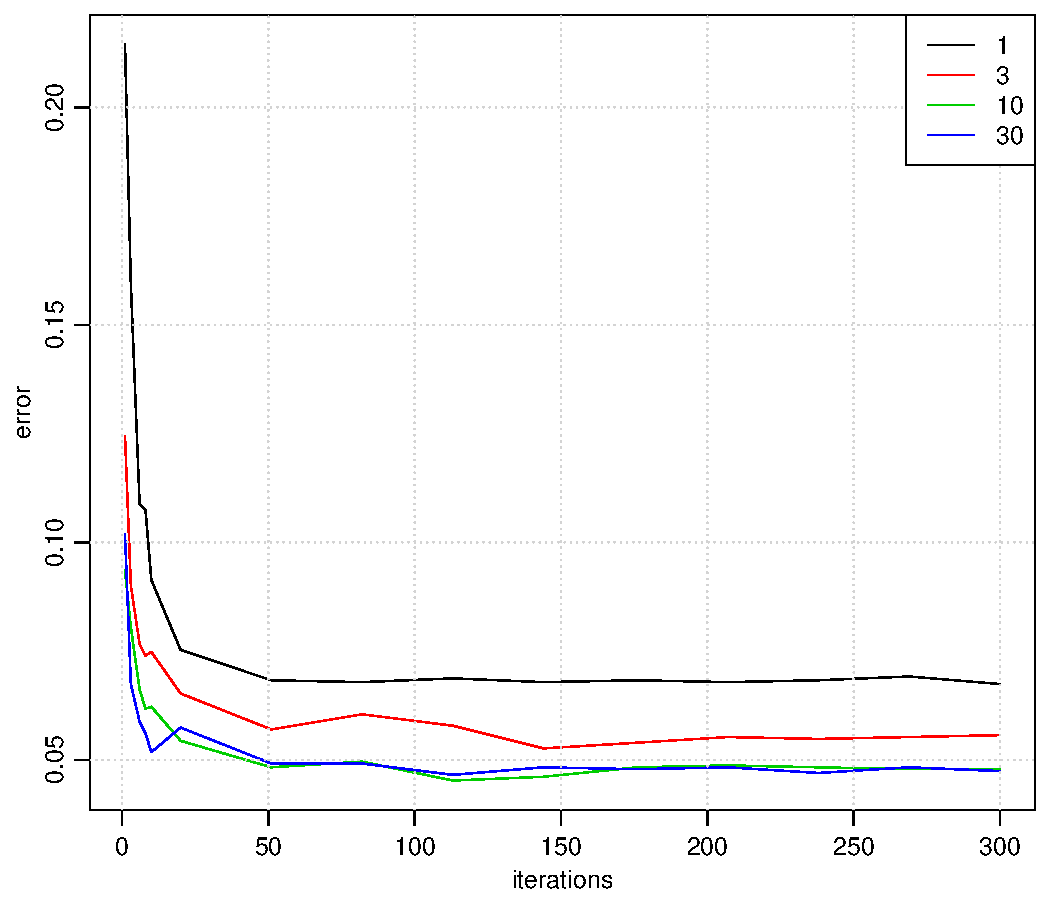
\includegraphics[scale=0.5]{./figures/adaboostSpam.pdf}
\end{center}
\caption{AdaBoost on spam data. For different tree depths.}
\label{fig:adaboostSpam}
\end{figure}

Simulation 2: \\
With and without bootstraping. Maybe include this in Simulation 1.

\subsection{Gradient boosting}
\label{sub:SimGradBoost}
\colorbox{yellow}{Both gradient and stochastic.}\\
\colorbox{yellow}{Problems with gbm. See tutorial}
\url{https://vimeo.com/71992876} \\
\url{http://www.datarobot.com/blog/r-getting-started-with-data-science/}
\\ \colorbox{yellow}{Should I include offset in the model?}
\\ \colorbox{yellow}{Make adaboost with gbm as good as with adabag}
\\ \colorbox{yellow}{Use gbm.fit, as it should be faster for ''power users''} \\
\url{http://www.saedsayad.com/docs/gbm2.pdf} \colorbox{yellow}{Guide to gbm package}\\
\\
Simulation 1:\\
Plot error as function of iterations. This should be done for different shrinkage parameters.\\
Consider plotting training error as well.\\
\\
\begin{figure}[h!]
\begin{center}
    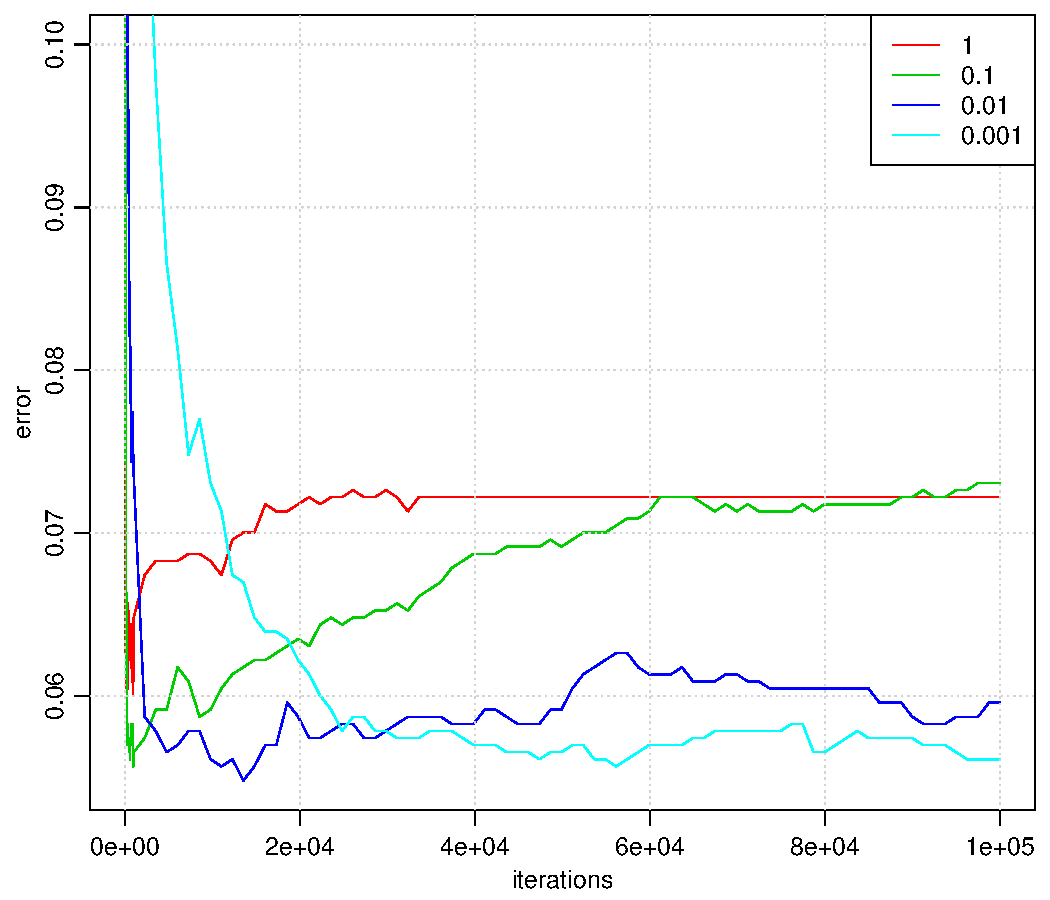
\includegraphics[scale=0.5]{./figures/gradboostSpamShrink2.pdf}
\end{center}
\caption{Gradient boosting on spam data. The shrinkage of each line is specified in the legend.}
\label{fig:gradboostSpamShrink2}
\end{figure}

Simulation 2:\\
Plot error as function of iterations, for different \verb+bag.fractions+, and report time for the different baggigs.\\
\\
\begin{figure}[h!]
  \centering
  \begin{subfigure}[b]{0.48\textwidth}
    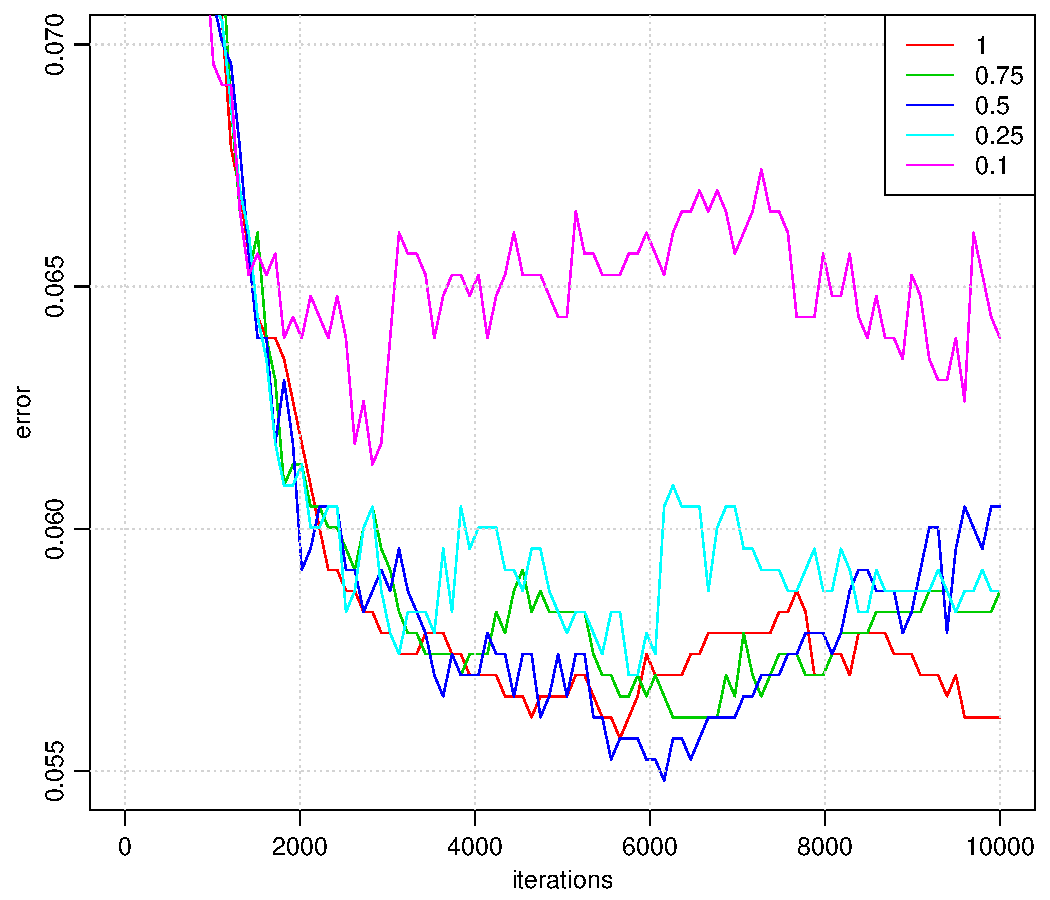
\includegraphics[width=\textwidth]{./figures/gradboostSpamStoch.pdf}
    \caption{Different bootstrap fractions.}
    \label{fig:gradboostSpamStoch}
  \end{subfigure}%
  \quad
  \begin{subfigure}[b]{0.48\textwidth}
    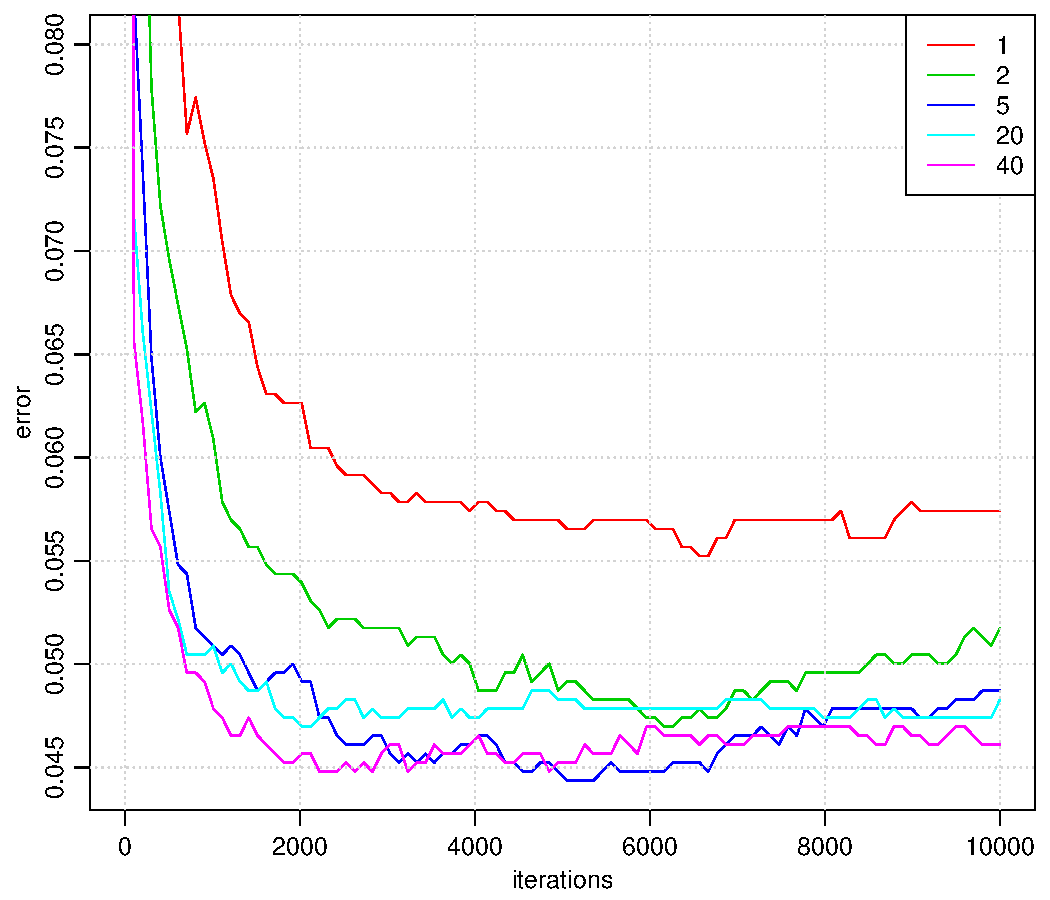
\includegraphics[width=\textwidth]{./figures/gradboostSpamDepth.pdf}
    \caption{Different tree depths.}
    \label{fig:gradboostSpamDepth}
  \end{subfigure}
          %(or a blank line to force the subfigure onto a new line)
  \vspace{1\baselineskip}
  \caption{Stochastic gradient boosting on spam data. Give some parameter values here!!!}
  \label{fig:StochasticGradBoost}
\end{figure}
\todo{parameters in Figure~\ref{fig:StochasticGradBoost}}
\colorbox{yellow}{Comment that there are unusually deep trees in Figure~\ref{fig:gradboostSpamDepth}}

Simulation 3:\\
Use \verb+interaction.depth+ (nr of splits) to set depth of tree, and see how that affect error as function of nr of iteratoins/trees.\\
\\ \colorbox{yellow}{Comment that not additive model as many nodes is better than stumps. See modstat.}
\\ \colorbox{yellow}{Figure~\ref{fig:gradboostSpamDepth}: see p.~13} \url{http://www.stat.cmu.edu/~ryantibs/datamining/lectures/25-boost.pdf}\\


\section{Bagging and Random Forest}
\label{sec:BaggandRFSim}
Simulation 1: \\
Do simulations for bagging with different bootstrap sizes. And the same for random forests\\
\\
\begin{figure}[h!]
  \centering
  \begin{subfigure}[b]{0.48\textwidth}
    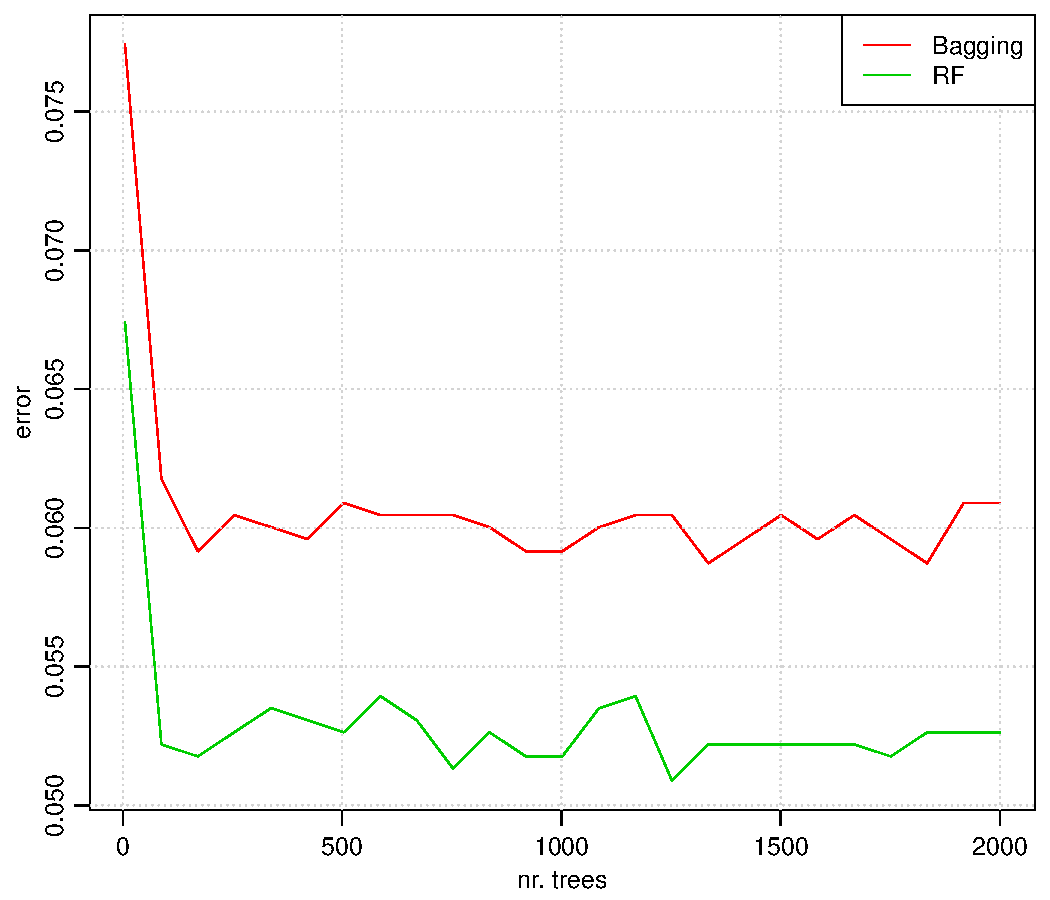
\includegraphics[width=\textwidth]{./figures/baggingAndRFSpam.pdf}
    \caption{Test error as function of bootstrap samples for bagging and RF.}
    \label{fig:baggingAndRFSpam}
  \end{subfigure}%
  \quad
  \begin{subfigure}[b]{0.48\textwidth}
    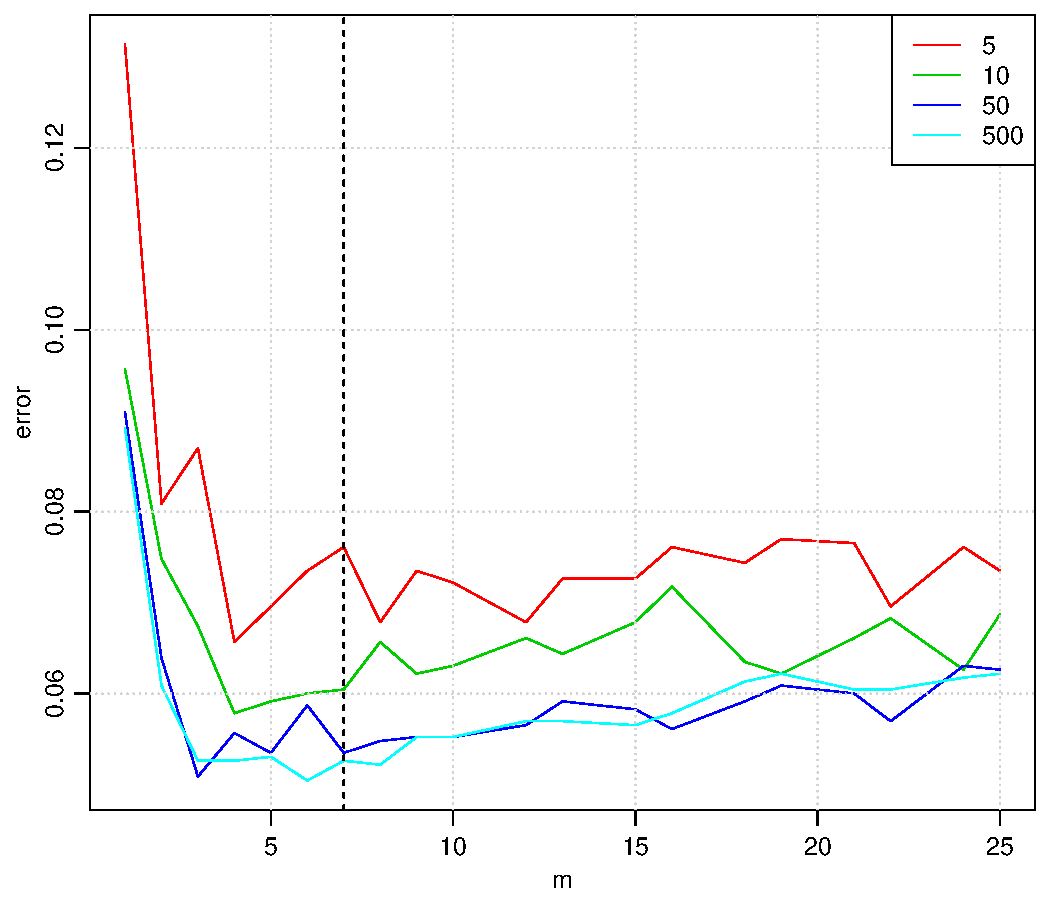
\includegraphics[width=\textwidth]{./figures/RFSpam.pdf}
    \caption{RF as func. of m, for different number of bootstrap samples. Vertical line marks $\sqrt{p}$.}
    \label{fig:RFSpam}
  \end{subfigure}
          %(or a blank line to force the subfigure onto a new line)
  \vspace{1\baselineskip}
  \caption{Misclassification rate for bagging and random forests on spam data.}
  \label{fig:baggAndRF}
\end{figure}
\todo{Comment on line in Figure~\ref{fig:RFSpam}}
\colorbox{yellow}{Comment how Figure~\ref{fig:baggingAndRFSpam} is many runs and not different iterations for one run.}
\\\colorbox{yellow}{That is why it is not smooth compared to Figure~\ref{fig:OOBvsTestvsCV}.}


Simulation 2: \\
\\
Maybe together with bagging, do simulations for as function of $m$'s, for different bootstrap sizes? \\
\colorbox{yellow}{Not sure what is best here.}\\
\\
\colorbox{yellow}{Comment that Figure~\ref{fig:baggingAndRFSpam} shows how RF don't overfit. Is the same true for bagging?}\\
\\
Simulation 3: \\
Show an example of when bagging and RF fails? If the base classifier is bad, then the aggregated can be bad as well.\\
\colorbox{yellow}{Should I do this?}\\
\\
\colorbox{yellow}{Do simulation to show diffenece between \eqref{eq:aggClass} and \eqref{eq:aggClassP}.}


\begin{figure}[h!]
\begin{center}
    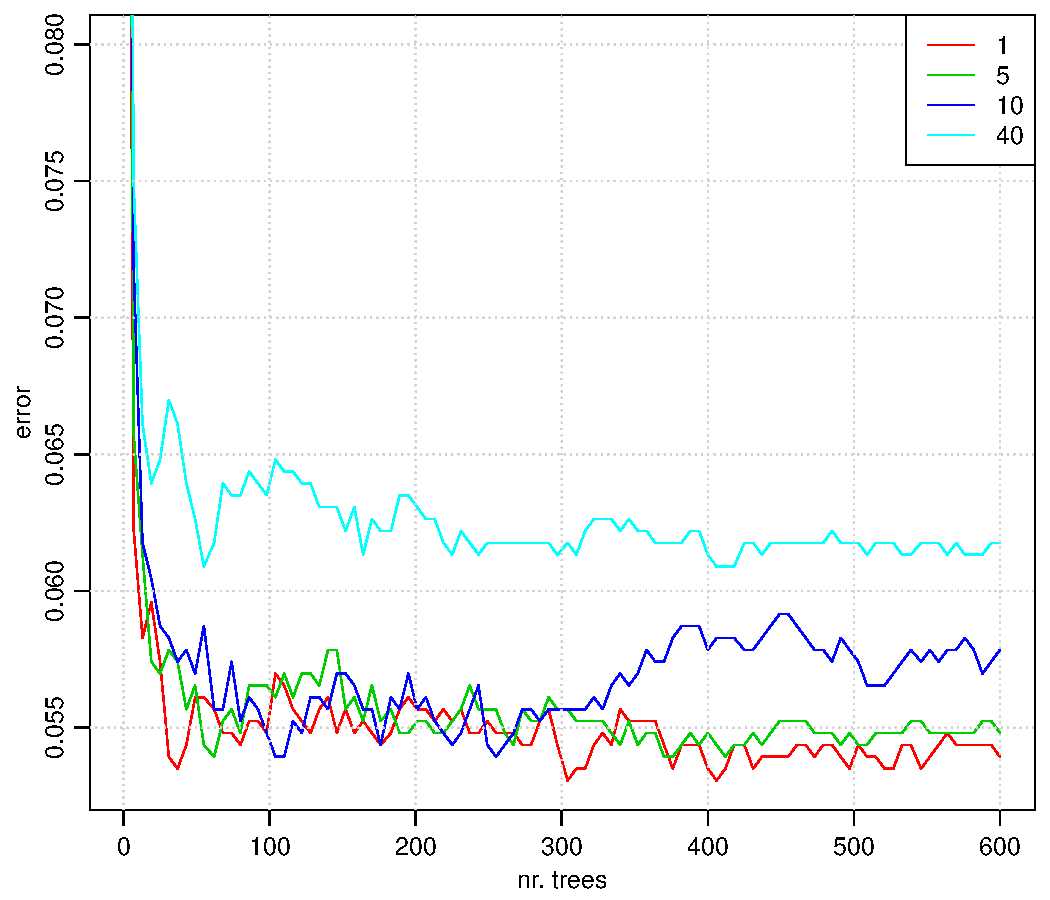
\includegraphics[scale=0.5]{./figures/RFTreeDepth.pdf}
\end{center}
\caption{Random forest on spam data, with different tree depths. The numbers in the legend indicates the minimum number of nodes in a terminal node.}
\label{fig:RFTreeDepth}
\end{figure}
\colorbox{yellow}{Benefits of not growing full sized trees is that it is faster, and some regularization.}


\begin{figure}[h!]
\begin{center}
    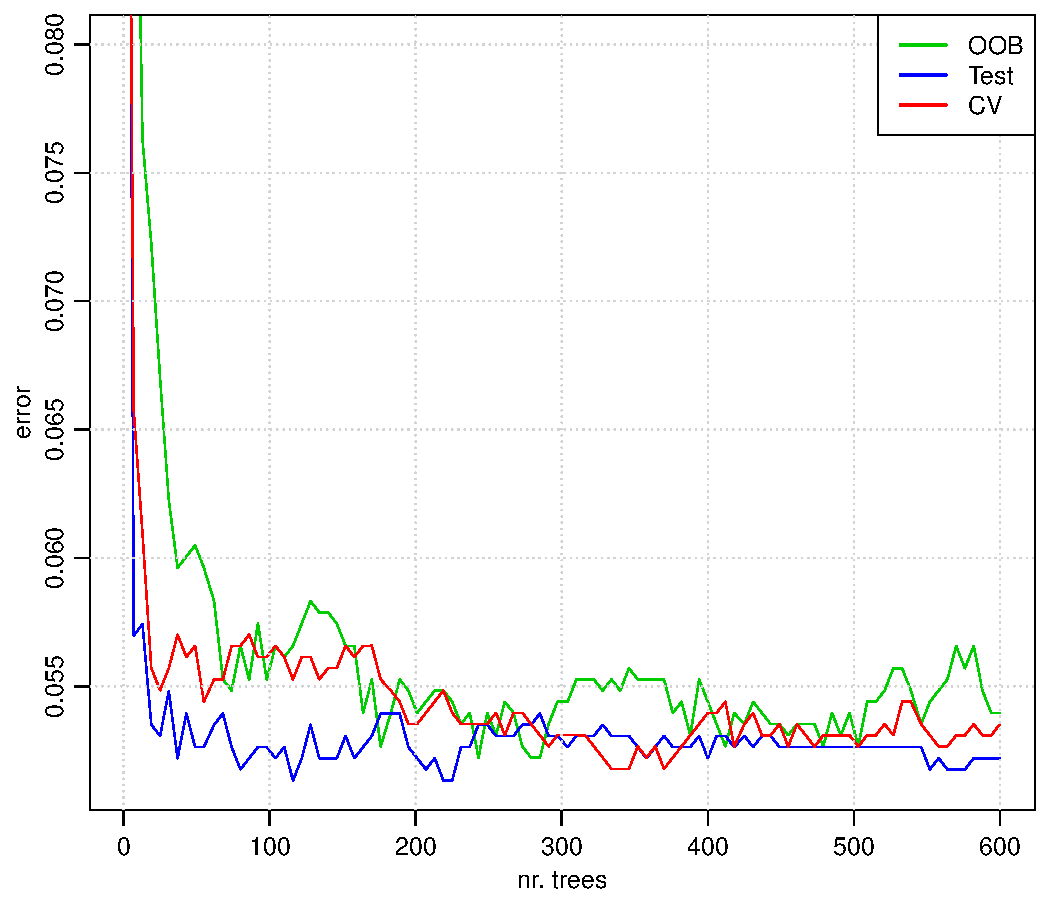
\includegraphics[scale=0.5]{./figures/OOBvsTestvsCV.pdf}
\end{center}
\caption{Out-of-bag, 10-fold cross-validation and test error for random forest on spam data.}
\label{fig:OOBvsTestvsCV}
\end{figure}
\colorbox{yellow}{Comment how they are very random, so Figure~\ref{fig:OOBvsTestvsCV} varies a lot.}\\






\section{Compare methods}
\label{sec:Compare methods}
\colorbox{yellow}{Show CART here as well.}

\subsection{Robustness}
\label{sub:Robustness}

\colorbox{yellow}{Add noise to previous test and see how stable the results are.}
\section{Phoneme}
\label{sec:Phoneme}
\begin{figure}[h!]
\begin{center}
    \includegraphics[scale=0.5]{./figures/cartCPPhoneme.pdf}
\end{center}
\caption{CART on Phoneme data.}
\label{fig:cartCPPhoneme}
\end{figure}


\begin{figure}[h!]
\begin{center}
    \includegraphics[scale=0.5]{./figures/adaboostPhoneme.pdf}
\end{center}
\caption{AdaBoost on Phoneme data. For different tree depths.}
\label{fig:adaboostPhoneme}
\end{figure}

\begin{figure}[h!]
\begin{center}
    \includegraphics[scale=0.5]{./figures/gradboostPhonemeShrink2.pdf}
\end{center}
\caption{Gradient boosting on Phoneme data. The shrinkage of each line is specified in the legend.}
\label{fig:gradboostPhonemeShrink2}
\end{figure}

\begin{figure}[h!]
  \centering
  \begin{subfigure}[b]{0.48\textwidth}
    \includegraphics[width=\textwidth]{./figures/gradboostPhonemeStoch.pdf}
    \caption{Different bootstrap fractions.}
    \label{fig:gradboostPhonemeStoch}
  \end{subfigure}%
  \quad
  \begin{subfigure}[b]{0.48\textwidth}
    \includegraphics[width=\textwidth]{./figures/gradboostPhonemeDepth.pdf}
    \caption{Different tree depths.}
    \label{fig:gradboostPhonemeDepth}
  \end{subfigure}
          %(or a blank line to force the subfigure onto a new line)
  \vspace{1\baselineskip}
  \caption{Stochastic gradient boosting on Phoneme data. Give some parameter values here!!!}
  \label{fig:StochasticGradBoostPhoneme}
\end{figure}

\begin{figure}[h!]
  \centering
  \begin{subfigure}[b]{0.48\textwidth}
    \includegraphics[width=\textwidth]{./figures/baggingAndRFPhoneme.pdf}
    \caption{Test error as function of bootstrap samples for bagging and RF.}
    \label{fig:baggingAndRFPhoneme}
  \end{subfigure}%
  \quad
  \begin{subfigure}[b]{0.48\textwidth}
    \includegraphics[width=\textwidth]{./figures/RFPhoneme.pdf}
    \caption{Test error for RF as function of m, for different number of bootstrap samples. Vertical line marks $\sqrt{p}$.}
    \label{fig:RFPhoneme}
  \end{subfigure}
          %(or a blank line to force the subfigure onto a new line)
  \vspace{1\baselineskip}
  \caption{Misclassification rate for bagging and random forests on Phoneme data.}
  \label{fig:baggAndRFPhoneme}
\end{figure}


\clearpage
\section{Needs to be done}
\label{sec:Needs to be done}
Write about deviance splitting in CART\\
\\
Do bagging/RF with probs instead of vote. (The two different methods in Bagging section). Write something about how p should be faster for B around 0.5.\\
\\
Write about categorical variables after simulation study. In modstat 9.2.4. discussion for CART\\
\\
Comment on how the timing is not particularly good. \\
\\
Comment on how a tree can be deep, but split on the same variable multiple times?\\
\\
Maybe repeat some of experiments with added noise?

\section{Questions}
\label{sec:Questions}
Should the bias-variance tradeoff be descussed before CART (as now), or inside the CART section?\\
\\
